\section*{ANEXOS} \label{sec:anexos} % Se añade un asterisco a \section para que el título no esté numerado.
\addcontentsline{toc}{section}{ANEXOS} % Al utilizar \section* se ha de añadir manualmente el apartado al índice (Table Of Contents, TOC).
\markright{ANEXOS} % Al utilizar \section* se ha de añadir manualmente el título del apartado al encabezado.

\renewcommand{\thesubsection}{\Alph{subsection}} % Se numeran los anexos con letras del alphabeto en lugar de números.
% Se indica que las tablas, figuras y códigos se numeran con el código del anexo (A, B, C, ...) seguido del número de tabla, figura o código dentro del anexo (tabla A.2, figura C.1, etc.)
\renewcommand{\thetable}{\Alph{subsection}.\arabic{table}}
\renewcommand{\thefigure}{\Alph{subsection}.\arabic{figure}}
\renewcommand{\thecode}{\Alph{subsection}.\arabic{code}}
\setcounter{subsection}{0} % Se reinicia el contador de anexos a 0.
% ---------------- Primer anexo ---------------- %
\subsection{Esquema de la base de datos} \label{sec:db_schema}

La tabla \ref{tab:db_schema} muestra el esquema de la base de datos relacional utilizada para almacenar los resultados de los experimentos realizados. Esta base de datos ha permitido organizar y estructurar la información obtenida durante el proceso de entrenamiento y evaluación de los modelos, facilitando su posterior análisis y comparación.

La organización de esta base de datos corresponde a tres tablas principales: \textbf{Runs\_t}, \textbf{Trials\_t} y \textbf{Classes\_t}. La tabla \textbf{Runs\_t} contiene información general sobre cada ejecución del experimento. La tabla \textbf{Trials\_t} almacena los resultados obtenidos durante la etapa de test de cada ejecución, separados por usuario, día y ensayo.

Finalmente, la tabla \textbf{Classes\_t} contiene los resultados de cada clase individual dentro de cada ensayo, esta tabla nos permite análizar el rendimiento del modelo en cada clase específica y evaluar su capacidad para diferenciar entre las distintas categorías presentes en el conjunto de datos. Se puede obtener así métricas adicionales como la tasa de falsos positivos y falsos negativos, que son fundamentales para comprender el comportamiento del modelo en situaciones de clasificación desequilibrada o cuando ciertas clases son más críticas que otras.

\begin{table}[H]
  \centering
  \begin{tabular}{|l|l|l|l|}
    \hline
    Nombre\_Tabla: & \textbf{Runs\_t}         & \textbf{Trials\_t }      & \textbf{Classes\_t}: \\ \hline
    N\_Entradas:   & 1917                     & 5751                     & 15336                \\ \hline
    \multicolumn{4}{|c|}{\textbf{Run metadata}}                                                 \\ \hline
    1              & run\_id                  & run\_id                  & run\_id              \\ \hline
    2              & run\_timestamp           & run\_timestamp           & run\_timestamp       \\ \hline
    3              & sample\_id               & sample\_id               & sample\_id           \\ \hline
    4              & title                    & ~                        & ~                    \\ \hline
    5              & file\_path               & ~                        & ~                    \\ \hline
    6              & comment                  & ~                        & ~                    \\ \hline
    \multicolumn{4}{|c|}{\textbf{Dimensions}}                                                   \\ \hline
    7              & training\_method         & training\_method         & training\_method     \\ \hline
    8              & model\_name              & model\_name              & model\_name          \\ \hline
    9              & task\_mode               & task\_mode               & task\_mode           \\ \hline
    10             & user                     & user                     & user                 \\ \hline
    11             & day                      & day                      & day                  \\ \hline
    12             & ~                        & trial\_id                & trial\_id            \\ \hline
    13             & ~                        & ~                        & class                \\ \hline
    \multicolumn{4}{|c|}{\textbf{Metrics}}                                                      \\ \hline
    14             & acc1                     & acc1                     & ~                    \\ \hline
    15             & val\_accuracy            & val\_accuracy            & ~                    \\ \hline
    16             & val\_precision\_macro    & val\_precision\_macro    & precision            \\ \hline
    17             & val\_recall\_macro       & val\_recall\_macro       & recall               \\ \hline
    18             & val\_f1\_macro           & val\_f1\_macro           & f1                   \\ \hline
    19             & val\_precision\_weighted & val\_precision\_weighted & ~                    \\ \hline
    20             & val\_recall\_weighted    & val\_recall\_weighted    & ~                    \\ \hline
    21             & val\_f1\_weighted        & val\_f1\_weighted        & support              \\ \hline
    22             & confusion\_matrix\_json  & confusion\_matrix\_json  & ~                    \\ \hline
    \multicolumn{4}{|c|}{\textbf{Training\_metrics:}}                                           \\ \hline
    27             & final\_train\_loss       & ~                        & ~                    \\ \hline
    28             & final\_train\_acc        & ~                        & ~                    \\ \hline
    29             & final\_training\_rate    & ~                        & ~                    \\ \hline
    30             & final\_val\_loss         & ~                        & ~                    \\ \hline
    31             & final\_val\_acc          & ~                        & ~                    \\ \hline
    32             & best\_epoch              & ~                        & ~                    \\ \hline
    33             & best\_val\_loss          & ~                        & ~                    \\ \hline
    34             & best\_val\_acc           & ~                        & ~                    \\ \hline
    \multicolumn{4}{|c|}{\textbf{Extras}}                                                       \\ \hline
    23             & training\_samples        & ~                        & ~                    \\ \hline
    24             & validation\_samples      & ~                        & ~                    \\ \hline
    25             & epochs\_planned          & ~                        & ~                    \\ \hline
    26             & epochs\_ran              & ~                        & ~                    \\ \hline
  \end{tabular}
  \caption{Esquema de la base de datos relacional utilizada para almacenar los resultados de los experimentos realizados.}
  \label{tab:db_schema}
\end{table}

\newpage

\subsection{Tablas complementarias de resultados}\label{sec:anexo_graficas}


\subsubsection{Tasa de falsos positivos y falsos negativos}
La tabla \ref{tab:false_positive_negative_rates} muestra un ejemplo de  las tasas de falsos positivos y falsos negativos para cada combinación de modelo y método de entrenamiento.

\begin{table}[!ht]
  \centering
  \begin{tabular}{|p{3em}|p{7em}|p{3cm}|p{3cm}|p{3cm}|}
    \hline
    \textbf{Task}              & \textbf{Model}                    & \textbf{Training Method} & \textbf{False Positive Rate}  & \textbf{False Negative Rate}  \\ \hline
    \multirow{12}{3em}{Motion} & \multirow{4}{7em}{DeepConvNet}    & Intra-Session            & \cellcolor[HTML]{F8CBAD}0.425 & \cellcolor[HTML]{FDEEE4}0.298 \\ \cline{3-5}
                               &                                   & Inter-Session            & \cellcolor[HTML]{F8CBAD}0.304 & \cellcolor[HTML]{F8CCAF}0.335 \\ \cline{3-5}
                               &                                   & Inter-Users              & \cellcolor[HTML]{FDF2EA}0.258 & \cellcolor[HTML]{F8CBAD}0.412 \\ \cline{3-5}
                               &                                   & Continuous               & \cellcolor[HTML]{FDEEE4}0.262 & \cellcolor[HTML]{F8CBAD}0.442 \\ \cline{2-5}
                               & \multirow{4}{4em}{EEGNet}         & Intra-Session            & \cellcolor[HTML]{FDFEFD}0.241 & \cellcolor[HTML]{FDEFE6}0.297 \\ \cline{3-5}
                               &                                   & Inter-Session            & \cellcolor[HTML]{FCEBDF}0.266 & \cellcolor[HTML]{F0FBF2}0.264 \\ \cline{3-5}
                               &                                   & Inter-Users              & \cellcolor[HTML]{FADDCA}0.280 & \cellcolor[HTML]{F9CFB3}0.332 \\ \cline{3-5}
                               &                                   & Continuous               & \cellcolor[HTML]{F8CBAD}0.302 & \cellcolor[HTML]{F8CBAD}0.337 \\ \cline{2-5}
                               & \multirow{4}{4em}{ShallowConvNet} & Intra-Session            & \cellcolor[HTML]{FDEFE6}0.261 & \cellcolor[HTML]{F4FCF6}0.268 \\ \cline{3-5}
                               &                                   & Inter-Session            & \cellcolor[HTML]{FFFEFD}0.245 & \cellcolor[HTML]{FDFEFD}0.277 \\ \cline{3-5}
                               &                                   & Inter-Users              & \cellcolor[HTML]{FDEFE6}0.261 & \cellcolor[HTML]{FDF3EC}0.292 \\ \cline{3-5}
                               &                                   & Continuous               & \cellcolor[HTML]{FBE4D5}0.273 & \cellcolor[HTML]{FADDCA}0.317 \\ \hline
    \multirow{12}{4em}{Static} & \multirow{4}{4em}{DeepConvNet}    & Intra-Session            & \cellcolor[HTML]{F9CFB4}0.296 & \cellcolor[HTML]{E3F7E7}0.249 \\ \cline{3-5}
                               &                                   & Inter-Session            & \cellcolor[HTML]{F3FCF5}0.232 & \cellcolor[HTML]{EDFAF0}0.260 \\ \cline{3-5}
                               &                                   & Inter-Users              & \cellcolor[HTML]{E7F8EB}0.220 & \cellcolor[HTML]{F5FCF6}0.269 \\ \cline{3-5}
                               &                                   & Continuous               & \cellcolor[HTML]{D9F4DE}0.205 & \cellcolor[HTML]{FBE4D4}0.310 \\ \cline{2-5}
                               & \multirow{4}{4em}{EEGNet}         & Intra-Session            & \cellcolor[HTML]{FEFFFE}0.242 & \cellcolor[HTML]{F0FBF2}0.263 \\ \cline{3-5}
                               &                                   & Inter-Session            & \cellcolor[HTML]{CAF0D1}0.189 & \cellcolor[HTML]{D2F2D8}0.231 \\ \cline{3-5}
                               &                                   & Inter-Users              & \cellcolor[HTML]{C6EFCE}0.184 & \cellcolor[HTML]{FDEDE3}0.299 \\ \cline{3-5}
                               &                                   & Continuous               & \cellcolor[HTML]{CEF1D5}0.194 & \cellcolor[HTML]{FFFDFB}0.282 \\ \cline{2-5}
                               & \multirow{4}{4em}{ShallowConvNet} & Intra-Session            & \cellcolor[HTML]{D7F4DD}0.203 & \cellcolor[HTML]{C6EFCE}0.209 \\ \cline{3-5}
                               &                                   & Inter-Session            & \cellcolor[HTML]{CCF1D3}0.191 & \cellcolor[HTML]{C6EFCE}0.206 \\ \cline{3-5}
                               &                                   & Inter-Users              & \cellcolor[HTML]{C6EFCE}0.180 & \cellcolor[HTML]{C6EFCE}0.218 \\ \cline{3-5}
                               &                                   & Continuous               & \cellcolor[HTML]{C6EFCE}0.180 & \cellcolor[HTML]{C8F0D0}0.221 \\ \hline
  \end{tabular}
  \caption{Tasas de falsos positivos y falsos negativos para cada combinación de modelo, método de entrenamiento y tarea objetivo. Los valores más altos se muestran en tonos rojizos, mientras que los valores más bajos se muestran en tonos verdosos.}
  \label{tab:false_positive_negative_rates}
\end{table}

\subsubsection{Precisión media y desviación estandar de cada usuario}

En la Tabla \ref{tab:mu_sd_users_task} se muestran las precisiones medias y desviaciones estándar de cada usuario separadas por tarea objetivo. La ultima fila agrupa las precisiones medias y desviaciones estándar de todos los usuarios.

\begin{table}[H]
  \centering
  \begin{tabular}{|l|l|l|l|}
    \hline
    user                            & task\_mode & mu                 & sd                  \\ \hline
    \multirow{2}{4em}{0}            & motion     & 0.6460258233       & 0.08461602092       \\ \cline{2-4}
                                    & static     & 0.7074175824       & 0.07006995298       \\ \hline
    \multirow{2}{4em}{1}            & motion     & 0.7646520147       & 0.142811407         \\ \cline{2-4}
                                    & static     & 0.8853010116       & 0.07966058612       \\ \hline
    \multirow{2}{4em}{2}            & motion     & 0.6313841599       & 0.11436005          \\ \cline{2-4}
                                    & static     & 0.600093985        & 0.1028584688        \\ \hline
    \multirow{2}{4em}{3}            & motion     & 0.6465894466       & 0.1249193032        \\ \cline{2-4}
                                    & static     & 0.8550125313       & 0.07263570034       \\ \hline
    \multirow{2}{4em}{4}            & motion     & 0.8097168597       & 0.1225040144        \\ \cline{2-4}
                                    & static     & 0.8335526316       & 0.09043700305       \\ \hline
    \multirow{2}{4em}{\textbf{All}} & motion     & 0.6988864889021312 & 0.13932102491049542 \\ \cline{2-4}
                                    & static     & 0.7762575802763694 & 0.13573189082767018 \\ \hline
  \end{tabular}
  \caption{Precisión media y desviación estándar por usuario y tarea.}
  \label{tab:mu_sd_users_task}
\end{table}

\subsubsection{Precisión media separada por tarea, método y modelo}

\begin{table}[!ht]
  \centering
  \begin{tabular}{|l|l|l|l|l|}
    \hline
    Método Entrenamiento              & Modelo         & Estática & Movimiento & Diferencia \\ \hline
    \multirow{3}{6em}{Intra-Sesión}   & DeepConvNet    & 0.70     & 0.63       & 0.07       \\ \cline{2-5}
                                      & EEGNet         & 0.70     & 0.68       & 0.02       \\ \cline{2-5}
                                      & ShallowConvNet & 0.79     & 0.73       & 0.06       \\ \hline
    \multirow{3}{6em}{Inter-Sesión}   & DeepConvNet    & 0.75     & 0.67       & 0.08       \\ \cline{2-5}
                                      & EEGNet         & 0.79     & 0.72       & 0.07       \\ \cline{2-5}
                                      & ShallowConvNet & 0.80     & 0.74       & 0.06       \\ \hline
    \multirow{3}{7em}{Inter-Usuarios} & DeepConvNet    & 0.76     & 0.66       & 0.10       \\ \cline{2-5}
                                      & EEGNet         & 0.76     & 0.68       & 0.09       \\ \cline{2-5}
                                      & ShallowConvNet & 0.81     & 0.73       & 0.07       \\ \hline
    \multirow{3}{6em}{Continuo}       & DeepConvNet    & 0.74     & 0.64       & 0.10       \\ \cline{2-5}
                                      & EEGNet         & 0.77     & 0.68       & 0.10       \\ \cline{2-5}
                                      & ShallowConvNet & 0.79     & 0.70       & 0.09       \\ \hline
    Diferencia Media                  &                &          &            & 0.07       \\ \hline
  \end{tabular}
\end{table}

\subsubsection{Evolución de la precisión por días separada por modelos}

Las figuras \ref{fig:user_day_variability_DeepConvNet}, \ref{fig:user_day_variability_ShallowConvNet} y \ref{fig:user_day_variability_EEGNet} muestran la evolución de la precisión por usuario y día para cada arquitectura.

Se pueden observar diferencias significativas en la evolución de la precisión entre los distintos usuarios y días, lo que indica que el rendimiento del modelo puede variar considerablemente dependiendo de los datos de entrenamiento y las condiciones específicas de cada usuario. Estas variaciones pueden deberse a factores individuales, como la calidad de la señal EEG, la fatiga del usuario o la familiaridad con la tarea, así como a factores externos, como el entorno de grabación o el equipo utilizado.

\begin{figure}[htbp]
  \centering
  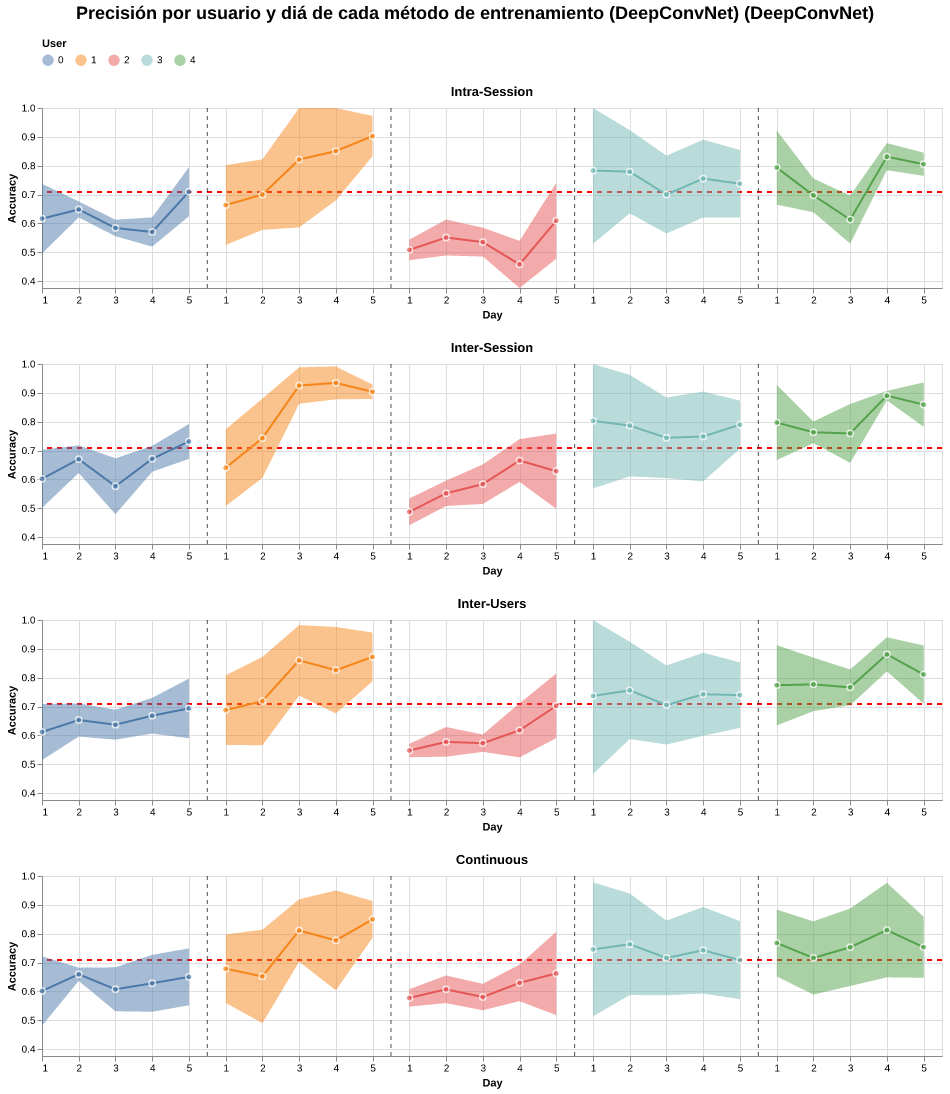
\includegraphics[width=1\textwidth]{img/resultados/Precision_por_usuario_y_dia_de_cada_metodo_de_entrenamiento_DeepConvNet_DeepConvNet.png}
  %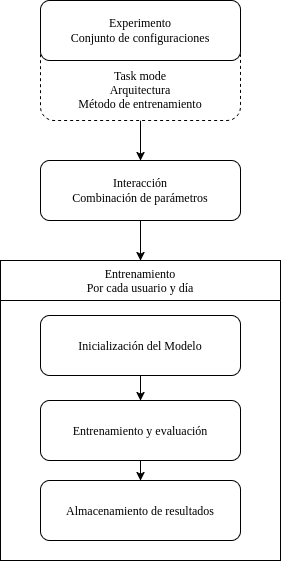
\includegraphics[height=\dimexpr\pagegoal-\pagetotal-\baselineskip\relax,width=\textwidth,keepaspectratio]{img/diagrama_pipeline.drawio.png}
  \caption{Variabilidad entre usuarios y día para cada método de entrenamiento para DeepConvNet.}
  \label{fig:user_day_variability_DeepConvNet}
\end{figure}

\begin{figure}[htbp]
  \centering
  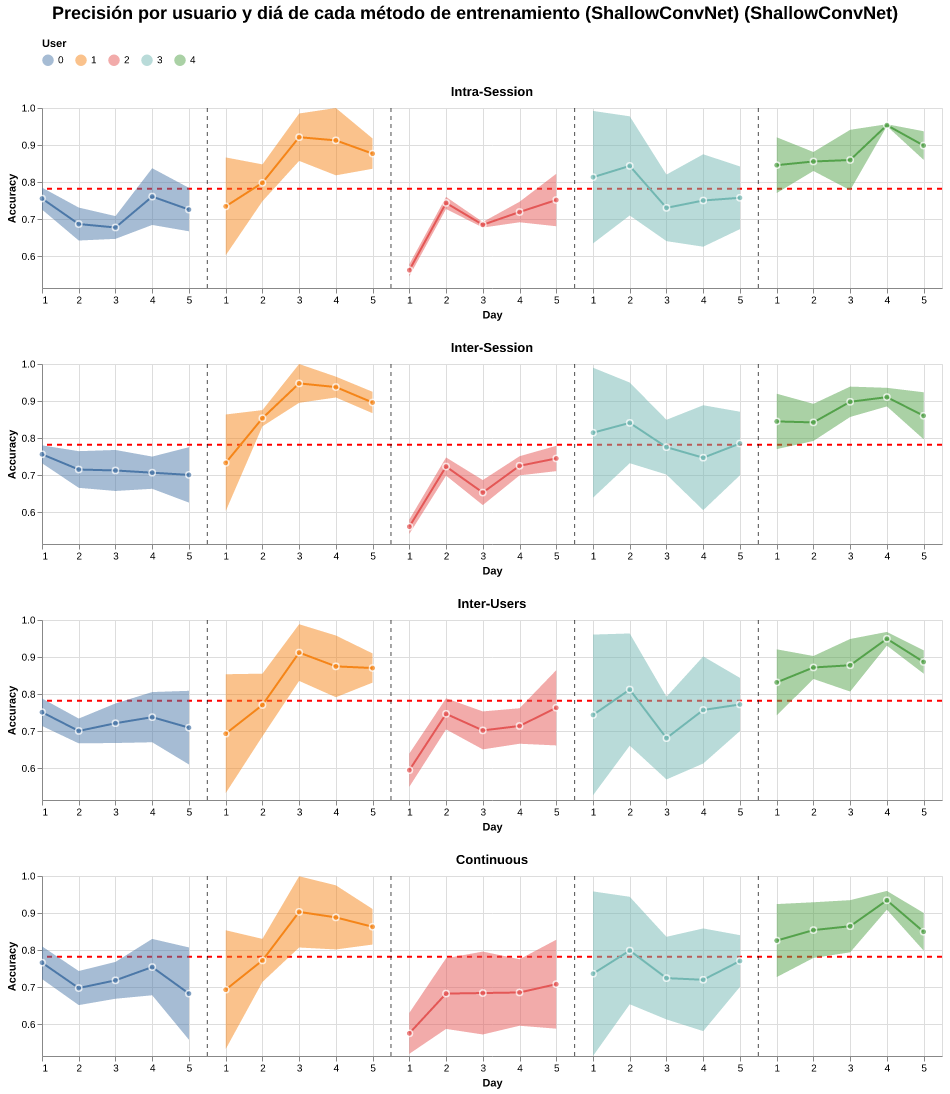
\includegraphics[width=1\textwidth]{img/resultados/Precision_por_usuario_y_dia_de_cada_metodo_de_entrenamiento_ShallowConvNet_ShallowConvNet.png}
  %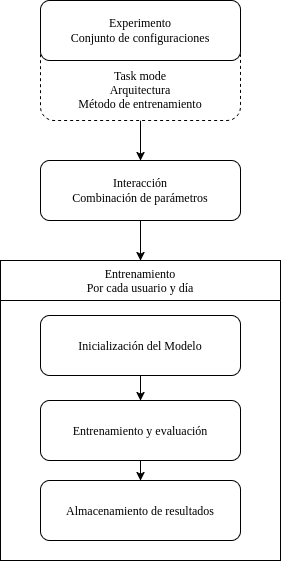
\includegraphics[height=\dimexpr\pagegoal-\pagetotal-\baselineskip\relax,width=\textwidth,keepaspectratio]{img/diagrama_pipeline.drawio.png}
  \caption{Variabilidad entre usuarios y día para cada método de entrenamiento para ShallowConvNet.}
  \label{fig:user_day_variability_ShallowConvNet}
\end{figure}

\begin{figure}[htbp]
  \centering
  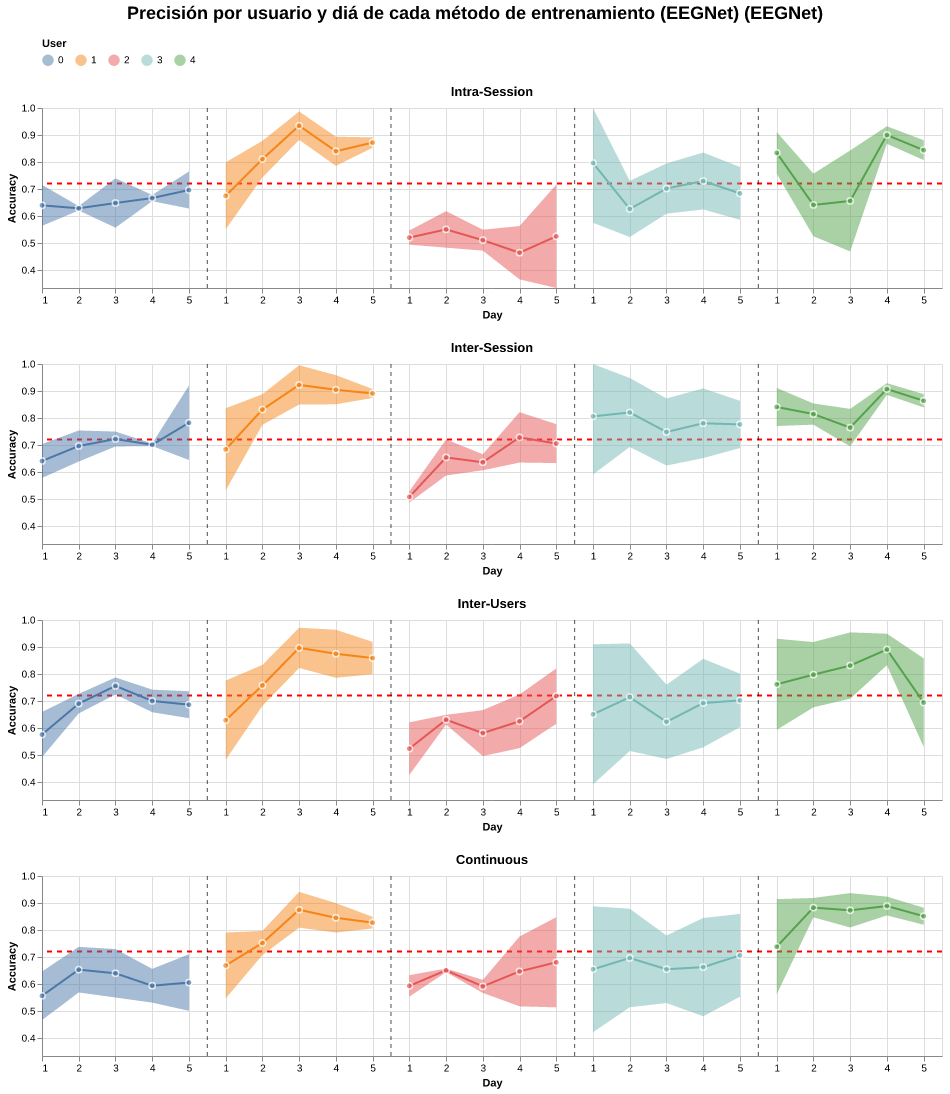
\includegraphics[width=1\textwidth]{img/resultados/Precision_por_usuario_y_dia_de_cada_metodo_de_entrenamiento_EEGNet_EEGNet.png}
  %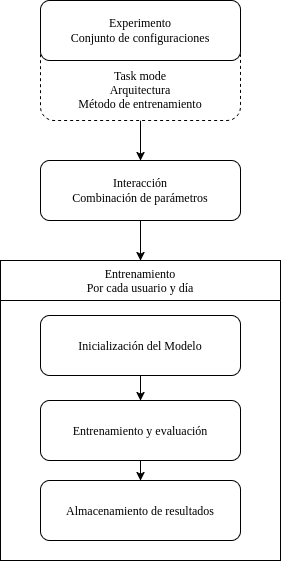
\includegraphics[height=\dimexpr\pagegoal-\pagetotal-\baselineskip\relax,width=\textwidth,keepaspectratio]{img/diagrama_pipeline.drawio.png}
  \caption{Variabilidad entre usuarios y día para cada método de entrenamiento para EEGNet.}
  \label{fig:user_day_variability_EEGNet}
\end{figure}


\newpage

\subsection{Queries complementarias}\label{sec:anexo_queries}

Con el objetivo de facilitar la reproducibilidad del análisis, el repositorio asociado al trabajo contiene las consultas SQL empleadas para obtener las tablas agregadas y generar las figuras presentadas en la memoria. En este anexo se incluyen las consultas principales, mientras que el conjunto completo puede consultarse en el directorio correspondiente del repositorio.

\subsubsection{Filtrado de Outliers}\label{sec:anexo_outliers}

Para realizar el filtrado de outliers utilizando el método Z-Score, se han definido nuevas vistas sobre cada una de las tablas \textbf{Runs\_t}, \textbf{Trials\_t} y \textbf{Classes\_t}. Manteniendo la estructura, pero eliminando valores atípicos. Además, se añaden los campos referentes a la configuración utilizada para el entrenamiento, de manera que se mantiene todo en la misma tabla.

Las queries utilizadas para la creación de las nuevas tablas ``limpias'' son las siguientes:

\begin{lstlisting}[
    style=sqlstyle,
    caption={Queries para la creación de las tablas ``limpias''.},
    label={cod:media_tarea}
]
CREATE
OR REPLACE VIEW runs_clean_z AS
WITH
    task_statistics AS (
        SELECT
            task_mode,
            AVG(acc1) AS mean_acc1,
            STDDEV_SAMP(acc1) AS std_acc1
        FROM
            runs_t
        WHERE
            acc1 IS NOT NULL
        GROUP BY
            task_mode
    )
SELECT
    t.*,
    p.*,
    (t.acc1 - s.mean_acc1) / NULLIF(s.std_acc1, 0) AS z_score
FROM
    runs_t AS t
    JOIN params_t AS p ON t.run_id = p.run_id
    JOIN task_statistics AS s ON t.task_mode = s.task_mode
WHERE
    t.acc1 IS NOT NULL
    AND t.acc1 <= 1
    AND ABS((t.acc1 - s.mean_acc1) / NULLIF(s.std_acc1, 0)) <= 3;

CREATE
OR REPLACE VIEW trials_clean_z AS
WITH
    task_statistics AS (
        SELECT
            task_mode,
            AVG(acc1) AS mean_acc1,
            STDDEV_SAMP(acc1) AS std_acc1
        FROM
            trials_t
        WHERE
            acc1 IS NOT NULL
        GROUP BY
            task_mode
    )
SELECT
    t.*,
    p.*,
    (t.acc1 - s.mean_acc1) / NULLIF(s.std_acc1, 0) AS z_score
FROM
    trials_t AS t
    JOIN params_t AS p ON t.run_id = p.run_id
    JOIN task_statistics AS s ON t.task_mode = s.task_mode
WHERE
    t.acc1 IS NOT NULL
    AND t.acc1 <= 1
    AND ABS((t.acc1 - s.mean_acc1) / NULLIF(s.std_acc1, 0)) <= 3;

CREATE
OR REPLACE VIEW classes_clean_z AS
WITH
    task_statistics AS (
        SELECT
            task_mode,
            AVG(precision) AS mean_acc1,
            STDDEV_SAMP(precision) AS std_acc1
        FROM
            classes_t
        WHERE
            precision IS NOT NULL
        GROUP BY
            task_mode
    )
SELECT
    t.*,
    p.*,
    (t.precision - s.mean_acc1) / NULLIF(s.std_acc1, 0) AS z_score
FROM
    classes_t AS t
    JOIN params_t AS p ON t.run_id = p.run_id
    JOIN task_statistics AS s ON t.task_mode = s.task_mode
WHERE
    t.precision IS NOT NULL
    AND t.precision <= 1
    AND ABS(
        (t.precision - s.mean_acc1) / NULLIF(s.std_acc1, 0)
    ) <= 3;
\end{lstlisting}


